\documentclass{article}
\usepackage[margin=1in]{geometry}
\usepackage[utf8]{inputenc}
\usepackage{graphicx} 
\usepackage{fancyhdr}
\usepackage{enumitem}
\usepackage{lipsum}
\usepackage[bahasa]{babel}
\usepackage{subcaption}
\usepackage{float}
\usepackage{indentfirst}

\title{Laporan Workshop Telematika \\ Dasar Desain Schematic dan PCB} % Ganti sesuai modul praktikum yang diikuti
\author{Azaria Putri Fawnia \\ 5024221038} % Ganti dengan NRP dan Nama Kalian

\date{}


\fancypagestyle{firstpageheader}{
  \fancyhf{} 
  \fancyhead[L]{
\includegraphics[height=1.5cm]{img/modul_1/logodepart.png}} 
  \fancyhead[R]{Institut Teknologi Sepuluh Nopember \\ Departemen Teknik Komputer \\ Laboratorium Robotika dan Sistem Cerdas} 
  \renewcommand{\headrulewidth}{0pt} 
  \fancyfoot[C]{%
    
\includegraphics[width=\textwidth]{img/modul_1/footer.png}
  }
  \renewcommand{\footrulewidth}{0pt} % No line in the footer
}


\fancyhf{} 
\fancyfoot[C]{%
  
\includegraphics[width=\textwidth]{img/modul_1/footer.png}
}
\renewcommand{\headrulewidth}{0pt} 
\renewcommand{\footrulewidth}{0pt} 

\pagestyle{fancy}
\begin{document}
\selectlanguage{bahasa}
\maketitle
\thispagestyle{firstpageheader}
% Bagian Tugas Pendahuluan
\section*{Tugas Pendahuluan}
\begin{enumerate}
  \item Jelaskan bagaimana cara kontrol 7-segment anoda dan katoda?
  \begin{enumerate}[label=\alph*.]
    \item 7-segment Anoda \\
    Pada display tujuh segmen dengan anoda umum, semua anoda dari segmen-segmen terhubung bersama, sementara setiap segmen memiliki koneksi katoda yang terpisah. Untuk menyalakan segmen tertentu, katoda segmen yang diinginkan dihubungkan ke ground, sementara tegangan positif dikirimkan ke anoda bersama, memungkinkan segmen tersebut untuk menyala pada saat yang bersamaan dengan segmen lain yang diinginkan.
    
    \item 7-segment Katoda \\
    Dalam display tujuh segmen dengan katoda umum, semua katoda dari segmen-segmen terhubung bersama, sementara setiap segmen memiliki koneksi anoda yang terpisah. Untuk menyalakan segmen tertentu, anoda segmen yang diinginkan dihubungkan ke sumber daya positif, sedangkan katoda bersama dihubungkan ke ground, memungkinkan segmen tersebut untuk menyala pada saat yang bersamaan dengan segmen lain yang diinginkan.
  \end{enumerate}
  \item Buat schematic untuk menampilkan nomor kelompok menggunakan dua 7-segment!
  pada folder praktikan \\
  \begin{figure}[H]
    \centering
    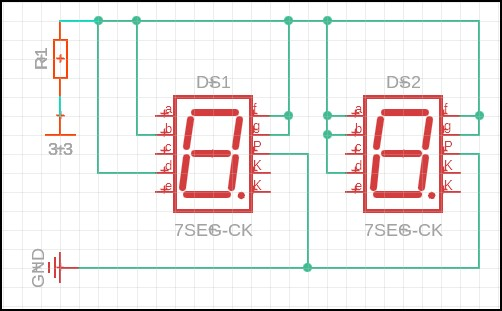
\includegraphics[width=0.6\linewidth]{img/modul_2/schematic_tupen2.jpg}
    \caption{Schematic sesuai nomor kelompok (13)} 
  \end{figure}
\end{enumerate}
% Bagian Analisis Hasil Percobaan
\section*{Analisis Hasil Percobaan}
\indent
Pada Percobaan modul 1 WORKSHOP Telematika, workshop dimulai dengan membuat rangkaian schematics minimum system ESP8266 yang dilakukan dengan mengikuti langkah-langkah yang sudah dicantumkan di modul. Proses membuat rangkaian schematic ini menggunakan komponen-komponen yang terdapat pada library yang sudah disediakan oleh aslab. Setelah proses membuar rangkaian schematic selesai, kemudian dibuat PCB dari schematic tersebut. Setelah proses wiring koneksi selesai kita mendapatkan hasil PCB yang siap di gunakan.



% \begin{table}[h]
%     \centering
%     \caption{Caption tabelnya}
%     \label{tab:labelini}
%     \begin{tabular}{|c|c|c|c|}
%     \hline
%     Kolom 1 & Kolom 2 & Kolom 3 & Kolom 4 \\
%     \hline
%     Data 1 & Data 2 & Data 3 & coba nambah kolom \\
%     Data 4 & Data 5 & Data 6 & coba nambah kolom juga \\ 
%     \hline
%     \end{tabular}
% \end{table}
% Bagian Lampiran
\section*{Lampiran} % Jika ada lampiran
\begin{figure}[H]
  \centering
  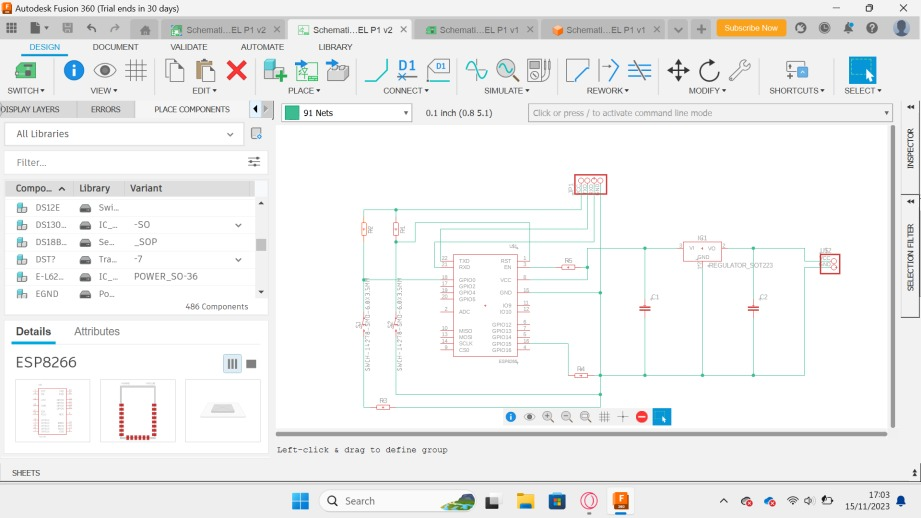
\includegraphics[width=0.7\linewidth]{img/modul_1/schematic.jpg}
  \caption{Membuat schematic} 
  \label{fig:inirujukan}
\end{figure}
\vspace{0pt}
\begin{figure}[H]
  \centering
  % Kalau mau menambah gambar lagi tinggal nambahin begin{subfigure} -> end{subfigure}
  \begin{subfigure}[b]{0.4\linewidth}
    \centering
    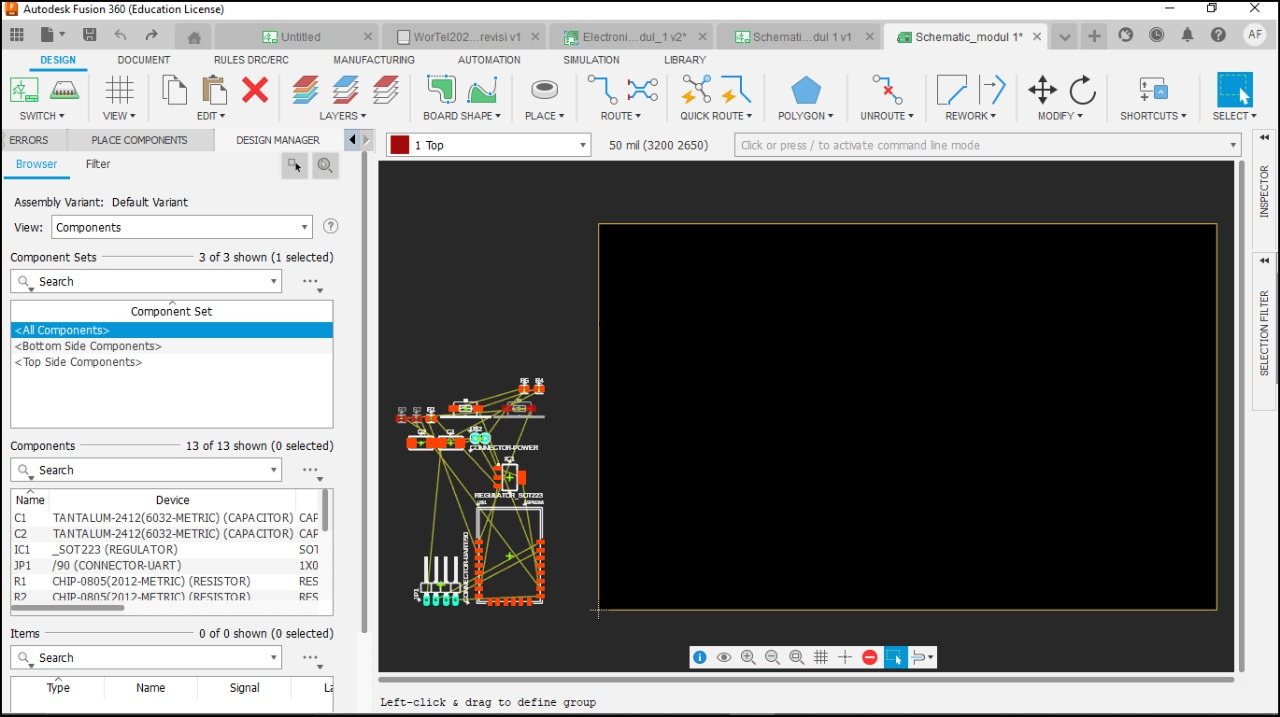
\includegraphics[width=\linewidth]{img/modul_1/circuit before1.jpeg}
    \caption{Komponen PCB sebelum dirangkai\label{fig:inisub1}}
  \end{subfigure}
  \hspace{1cm}
  \begin{subfigure}[b]{0.4\linewidth}
    \centering
    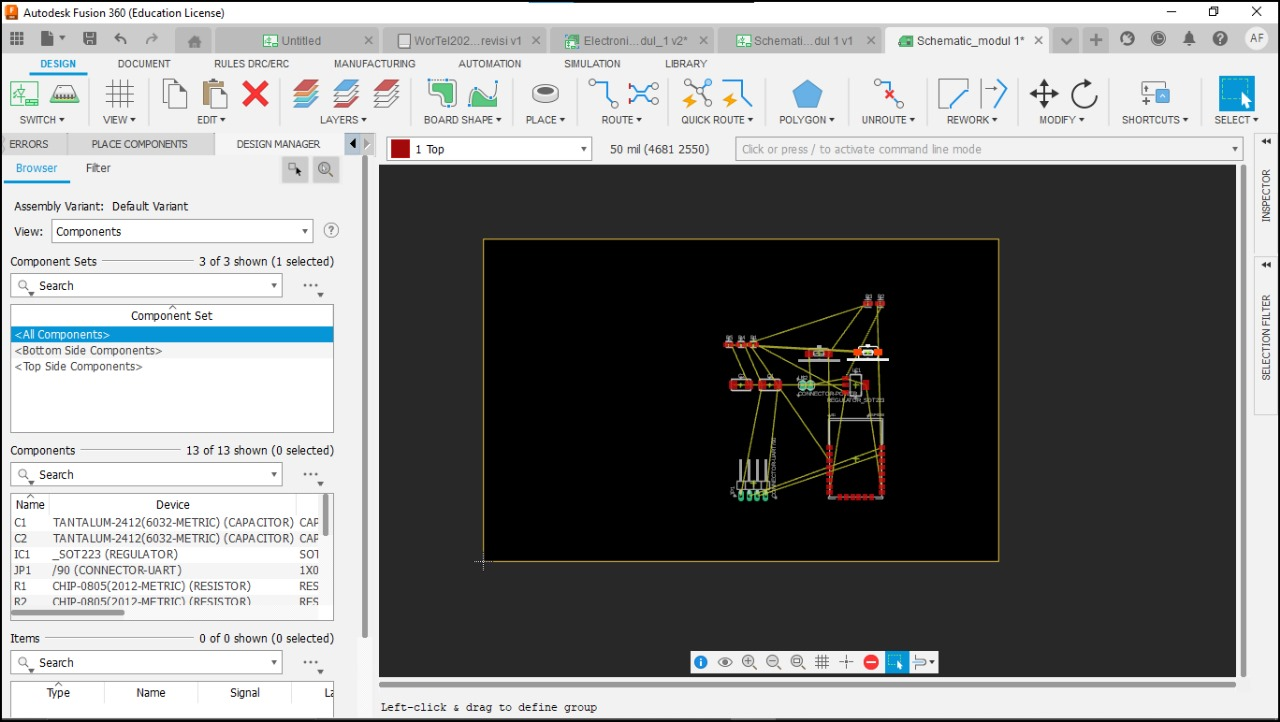
\includegraphics[width=\linewidth]{img/modul_1/circuit before.jpeg}
    \caption{Mulai merangkai PCB\label{fig:inisub2}}
  \end{subfigure}
  \caption{Proses merangkai PCB\label{fig:keduagambar}}
\end{figure}

\begin{figure}[H]
  \centering
  % Kalau mau menambah gambar lagi tinggal nambahin begin{subfigure} -> end{subfigure}
  \begin{subfigure}[c]{0.4\linewidth}
    \centering
    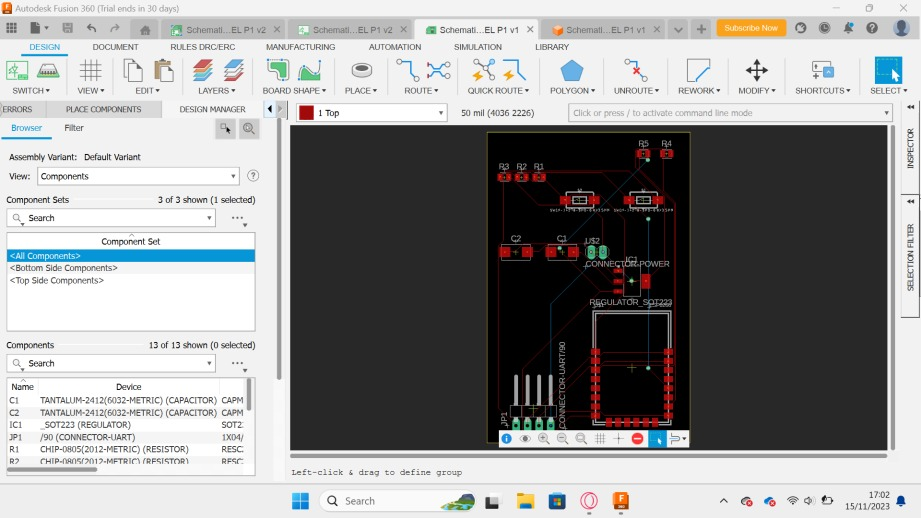
\includegraphics[width=\linewidth]{img/modul_1/PCB DONE.jpeg}
    \caption{Routing complete\label{fig:inisub1}}
  \end{subfigure}
  \hspace{1cm}
  \begin{subfigure}[c]{0.4\linewidth}
    \centering
    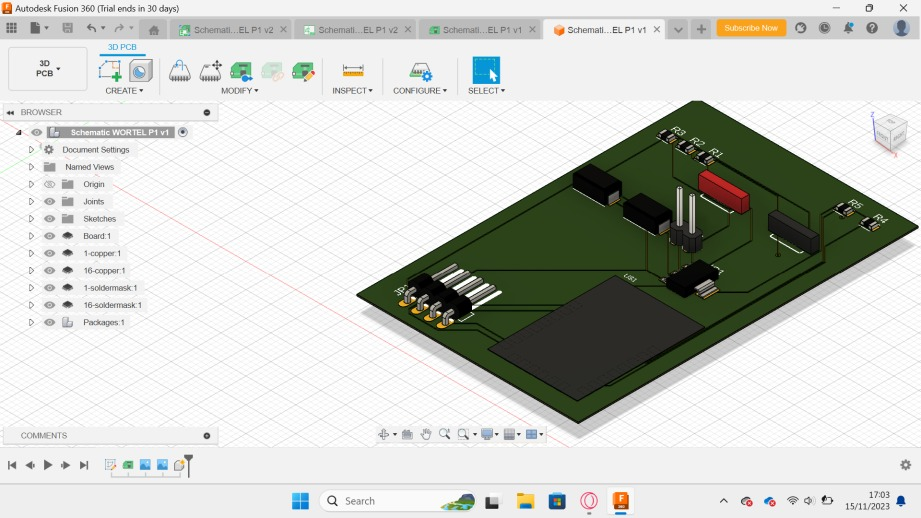
\includegraphics[width=\linewidth]{img/modul_1/3D Model.jpeg}
    \caption{visualisasi 3D dari PCB\label{fig:inisub2}}
  \end{subfigure}
  \caption{Hasil\label{fig:keduagambar}}
\end{figure}
\end{document}